% Options for packages loaded elsewhere
\PassOptionsToPackage{unicode}{hyperref}
\PassOptionsToPackage{hyphens}{url}
\PassOptionsToPackage{dvipsnames,svgnames,x11names}{xcolor}
%
\documentclass[
  letterpaper,
  DIV=11,
  numbers=noendperiod]{scrartcl}

\usepackage{amsmath,amssymb}
\usepackage{iftex}
\ifPDFTeX
  \usepackage[T1]{fontenc}
  \usepackage[utf8]{inputenc}
  \usepackage{textcomp} % provide euro and other symbols
\else % if luatex or xetex
  \usepackage{unicode-math}
  \defaultfontfeatures{Scale=MatchLowercase}
  \defaultfontfeatures[\rmfamily]{Ligatures=TeX,Scale=1}
\fi
\usepackage{lmodern}
\ifPDFTeX\else  
    % xetex/luatex font selection
\fi
% Use upquote if available, for straight quotes in verbatim environments
\IfFileExists{upquote.sty}{\usepackage{upquote}}{}
\IfFileExists{microtype.sty}{% use microtype if available
  \usepackage[]{microtype}
  \UseMicrotypeSet[protrusion]{basicmath} % disable protrusion for tt fonts
}{}
\makeatletter
\@ifundefined{KOMAClassName}{% if non-KOMA class
  \IfFileExists{parskip.sty}{%
    \usepackage{parskip}
  }{% else
    \setlength{\parindent}{0pt}
    \setlength{\parskip}{6pt plus 2pt minus 1pt}}
}{% if KOMA class
  \KOMAoptions{parskip=half}}
\makeatother
\usepackage{xcolor}
\setlength{\emergencystretch}{3em} % prevent overfull lines
\setcounter{secnumdepth}{-\maxdimen} % remove section numbering
% Make \paragraph and \subparagraph free-standing
\makeatletter
\ifx\paragraph\undefined\else
  \let\oldparagraph\paragraph
  \renewcommand{\paragraph}{
    \@ifstar
      \xxxParagraphStar
      \xxxParagraphNoStar
  }
  \newcommand{\xxxParagraphStar}[1]{\oldparagraph*{#1}\mbox{}}
  \newcommand{\xxxParagraphNoStar}[1]{\oldparagraph{#1}\mbox{}}
\fi
\ifx\subparagraph\undefined\else
  \let\oldsubparagraph\subparagraph
  \renewcommand{\subparagraph}{
    \@ifstar
      \xxxSubParagraphStar
      \xxxSubParagraphNoStar
  }
  \newcommand{\xxxSubParagraphStar}[1]{\oldsubparagraph*{#1}\mbox{}}
  \newcommand{\xxxSubParagraphNoStar}[1]{\oldsubparagraph{#1}\mbox{}}
\fi
\makeatother

\usepackage{color}
\usepackage{fancyvrb}
\newcommand{\VerbBar}{|}
\newcommand{\VERB}{\Verb[commandchars=\\\{\}]}
\DefineVerbatimEnvironment{Highlighting}{Verbatim}{commandchars=\\\{\}}
% Add ',fontsize=\small' for more characters per line
\usepackage{framed}
\definecolor{shadecolor}{RGB}{241,243,245}
\newenvironment{Shaded}{\begin{snugshade}}{\end{snugshade}}
\newcommand{\AlertTok}[1]{\textcolor[rgb]{0.68,0.00,0.00}{#1}}
\newcommand{\AnnotationTok}[1]{\textcolor[rgb]{0.37,0.37,0.37}{#1}}
\newcommand{\AttributeTok}[1]{\textcolor[rgb]{0.40,0.45,0.13}{#1}}
\newcommand{\BaseNTok}[1]{\textcolor[rgb]{0.68,0.00,0.00}{#1}}
\newcommand{\BuiltInTok}[1]{\textcolor[rgb]{0.00,0.23,0.31}{#1}}
\newcommand{\CharTok}[1]{\textcolor[rgb]{0.13,0.47,0.30}{#1}}
\newcommand{\CommentTok}[1]{\textcolor[rgb]{0.37,0.37,0.37}{#1}}
\newcommand{\CommentVarTok}[1]{\textcolor[rgb]{0.37,0.37,0.37}{\textit{#1}}}
\newcommand{\ConstantTok}[1]{\textcolor[rgb]{0.56,0.35,0.01}{#1}}
\newcommand{\ControlFlowTok}[1]{\textcolor[rgb]{0.00,0.23,0.31}{\textbf{#1}}}
\newcommand{\DataTypeTok}[1]{\textcolor[rgb]{0.68,0.00,0.00}{#1}}
\newcommand{\DecValTok}[1]{\textcolor[rgb]{0.68,0.00,0.00}{#1}}
\newcommand{\DocumentationTok}[1]{\textcolor[rgb]{0.37,0.37,0.37}{\textit{#1}}}
\newcommand{\ErrorTok}[1]{\textcolor[rgb]{0.68,0.00,0.00}{#1}}
\newcommand{\ExtensionTok}[1]{\textcolor[rgb]{0.00,0.23,0.31}{#1}}
\newcommand{\FloatTok}[1]{\textcolor[rgb]{0.68,0.00,0.00}{#1}}
\newcommand{\FunctionTok}[1]{\textcolor[rgb]{0.28,0.35,0.67}{#1}}
\newcommand{\ImportTok}[1]{\textcolor[rgb]{0.00,0.46,0.62}{#1}}
\newcommand{\InformationTok}[1]{\textcolor[rgb]{0.37,0.37,0.37}{#1}}
\newcommand{\KeywordTok}[1]{\textcolor[rgb]{0.00,0.23,0.31}{\textbf{#1}}}
\newcommand{\NormalTok}[1]{\textcolor[rgb]{0.00,0.23,0.31}{#1}}
\newcommand{\OperatorTok}[1]{\textcolor[rgb]{0.37,0.37,0.37}{#1}}
\newcommand{\OtherTok}[1]{\textcolor[rgb]{0.00,0.23,0.31}{#1}}
\newcommand{\PreprocessorTok}[1]{\textcolor[rgb]{0.68,0.00,0.00}{#1}}
\newcommand{\RegionMarkerTok}[1]{\textcolor[rgb]{0.00,0.23,0.31}{#1}}
\newcommand{\SpecialCharTok}[1]{\textcolor[rgb]{0.37,0.37,0.37}{#1}}
\newcommand{\SpecialStringTok}[1]{\textcolor[rgb]{0.13,0.47,0.30}{#1}}
\newcommand{\StringTok}[1]{\textcolor[rgb]{0.13,0.47,0.30}{#1}}
\newcommand{\VariableTok}[1]{\textcolor[rgb]{0.07,0.07,0.07}{#1}}
\newcommand{\VerbatimStringTok}[1]{\textcolor[rgb]{0.13,0.47,0.30}{#1}}
\newcommand{\WarningTok}[1]{\textcolor[rgb]{0.37,0.37,0.37}{\textit{#1}}}

\providecommand{\tightlist}{%
  \setlength{\itemsep}{0pt}\setlength{\parskip}{0pt}}\usepackage{longtable,booktabs,array}
\usepackage{calc} % for calculating minipage widths
% Correct order of tables after \paragraph or \subparagraph
\usepackage{etoolbox}
\makeatletter
\patchcmd\longtable{\par}{\if@noskipsec\mbox{}\fi\par}{}{}
\makeatother
% Allow footnotes in longtable head/foot
\IfFileExists{footnotehyper.sty}{\usepackage{footnotehyper}}{\usepackage{footnote}}
\makesavenoteenv{longtable}
\usepackage{graphicx}
\makeatletter
\def\maxwidth{\ifdim\Gin@nat@width>\linewidth\linewidth\else\Gin@nat@width\fi}
\def\maxheight{\ifdim\Gin@nat@height>\textheight\textheight\else\Gin@nat@height\fi}
\makeatother
% Scale images if necessary, so that they will not overflow the page
% margins by default, and it is still possible to overwrite the defaults
% using explicit options in \includegraphics[width, height, ...]{}
\setkeys{Gin}{width=\maxwidth,height=\maxheight,keepaspectratio}
% Set default figure placement to htbp
\makeatletter
\def\fps@figure{htbp}
\makeatother

\KOMAoption{captions}{tableheading}
\makeatletter
\@ifpackageloaded{caption}{}{\usepackage{caption}}
\AtBeginDocument{%
\ifdefined\contentsname
  \renewcommand*\contentsname{Table of contents}
\else
  \newcommand\contentsname{Table of contents}
\fi
\ifdefined\listfigurename
  \renewcommand*\listfigurename{List of Figures}
\else
  \newcommand\listfigurename{List of Figures}
\fi
\ifdefined\listtablename
  \renewcommand*\listtablename{List of Tables}
\else
  \newcommand\listtablename{List of Tables}
\fi
\ifdefined\figurename
  \renewcommand*\figurename{Figure}
\else
  \newcommand\figurename{Figure}
\fi
\ifdefined\tablename
  \renewcommand*\tablename{Table}
\else
  \newcommand\tablename{Table}
\fi
}
\@ifpackageloaded{float}{}{\usepackage{float}}
\floatstyle{ruled}
\@ifundefined{c@chapter}{\newfloat{codelisting}{h}{lop}}{\newfloat{codelisting}{h}{lop}[chapter]}
\floatname{codelisting}{Listing}
\newcommand*\listoflistings{\listof{codelisting}{List of Listings}}
\makeatother
\makeatletter
\makeatother
\makeatletter
\@ifpackageloaded{caption}{}{\usepackage{caption}}
\@ifpackageloaded{subcaption}{}{\usepackage{subcaption}}
\makeatother

\ifLuaTeX
  \usepackage{selnolig}  % disable illegal ligatures
\fi
\usepackage{bookmark}

\IfFileExists{xurl.sty}{\usepackage{xurl}}{} % add URL line breaks if available
\urlstyle{same} % disable monospaced font for URLs
\hypersetup{
  pdftitle={i-Plus User Guide},
  pdfauthor={Amelia Babb; Teddy Martin; Mags McLaughlin; Tillie Slosser},
  colorlinks=true,
  linkcolor={blue},
  filecolor={Maroon},
  citecolor={Blue},
  urlcolor={Blue},
  pdfcreator={LaTeX via pandoc}}


\title{i-Plus User Guide}
\author{Amelia Babb \and Teddy Martin \and Mags McLaughlin \and Tillie
Slosser}
\date{}

\begin{document}
\maketitle


\subsection{Introduction}\label{introduction}

i-Plus is a tool developed by students in SDS 410: Capstone in
Statistical \& Data Sciences for Elmhurst United Middle School. This
tool is integrated into Google Sheets using Google Apps Scripts and
allows for easier and more customizable visualization of data provided
by the i-Ready testing program. The steps to install i-Plus into Google
Sheets containing student data from Elmhurst are detailed in the
\textbf{Installing i-Plus} section of this user guide. Additionally,
certain data management practices are required to keep i-Plus
functioning properly. These steps are described in the \textbf{Data
Management} section of this guide. The most common error that arises
when running i-Plus is described in the \textbf{Common Errors} section
of this guide.

\subsection{Installing i-Plus}\label{installing-i-plus}

\begin{enumerate}
\def\labelenumi{\arabic{enumi}.}
\tightlist
\item
  Access Google Apps Scripts by navigating to \textbf{Extensions
  \textgreater{} Apps Script} within the sheet you want to add i-Plus to
\end{enumerate}

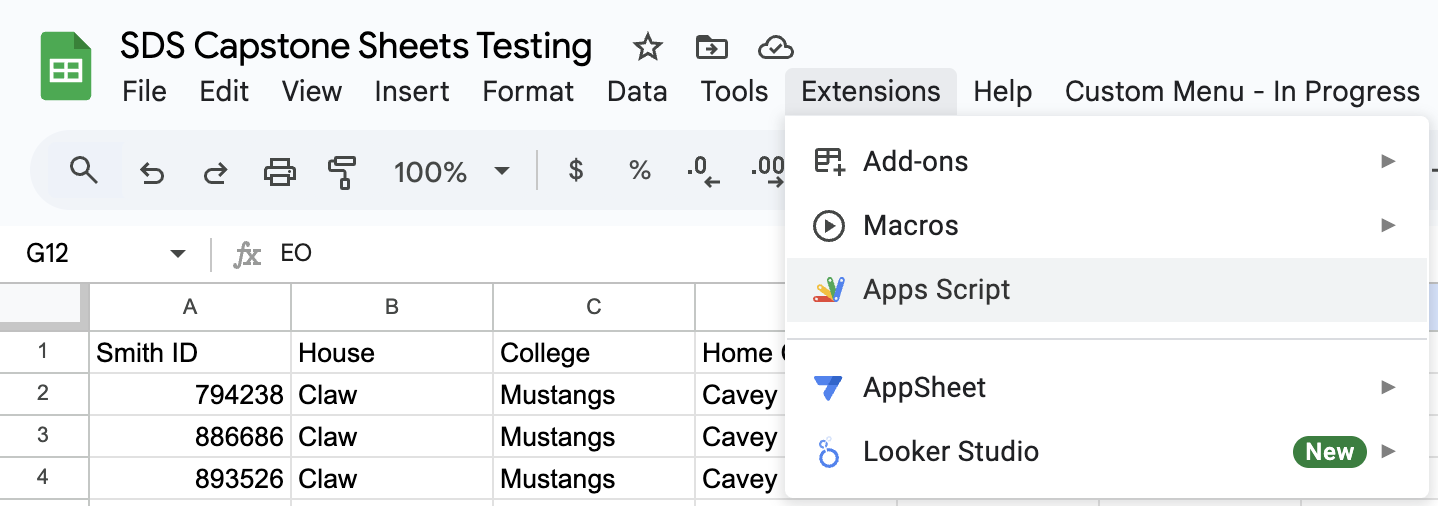
\includegraphics{images/image1.pdf}

\begin{enumerate}
\def\labelenumi{\arabic{enumi}.}
\setcounter{enumi}{1}
\tightlist
\item
  Access the library menu by choosing the plus button next to
  \textbf{Libraries} within the side menu of the Scripts window
\end{enumerate}

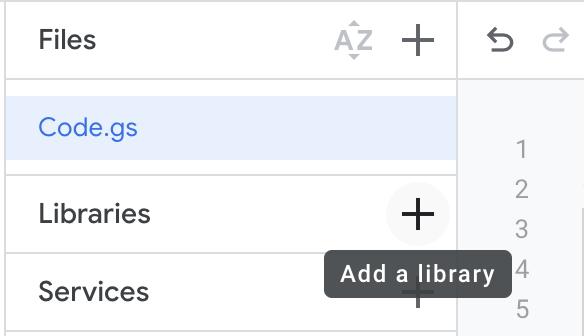
\includegraphics{/images/image2.pdf}

\begin{enumerate}
\def\labelenumi{\arabic{enumi}.}
\setcounter{enumi}{2}
\tightlist
\item
  Locate the i-Plus library by pasting the following code into the
  \textbf{Script ID} and selecting look up
\end{enumerate}

\begin{Shaded}
\begin{Highlighting}[]
\DecValTok{1}\NormalTok{os5M3\_htGWveLyoZGitnTZD3SnwptfRWwul15TmaodITFAuO\_6\_M4}\DecValTok{{-}3}\NormalTok{w}
\end{Highlighting}
\end{Shaded}

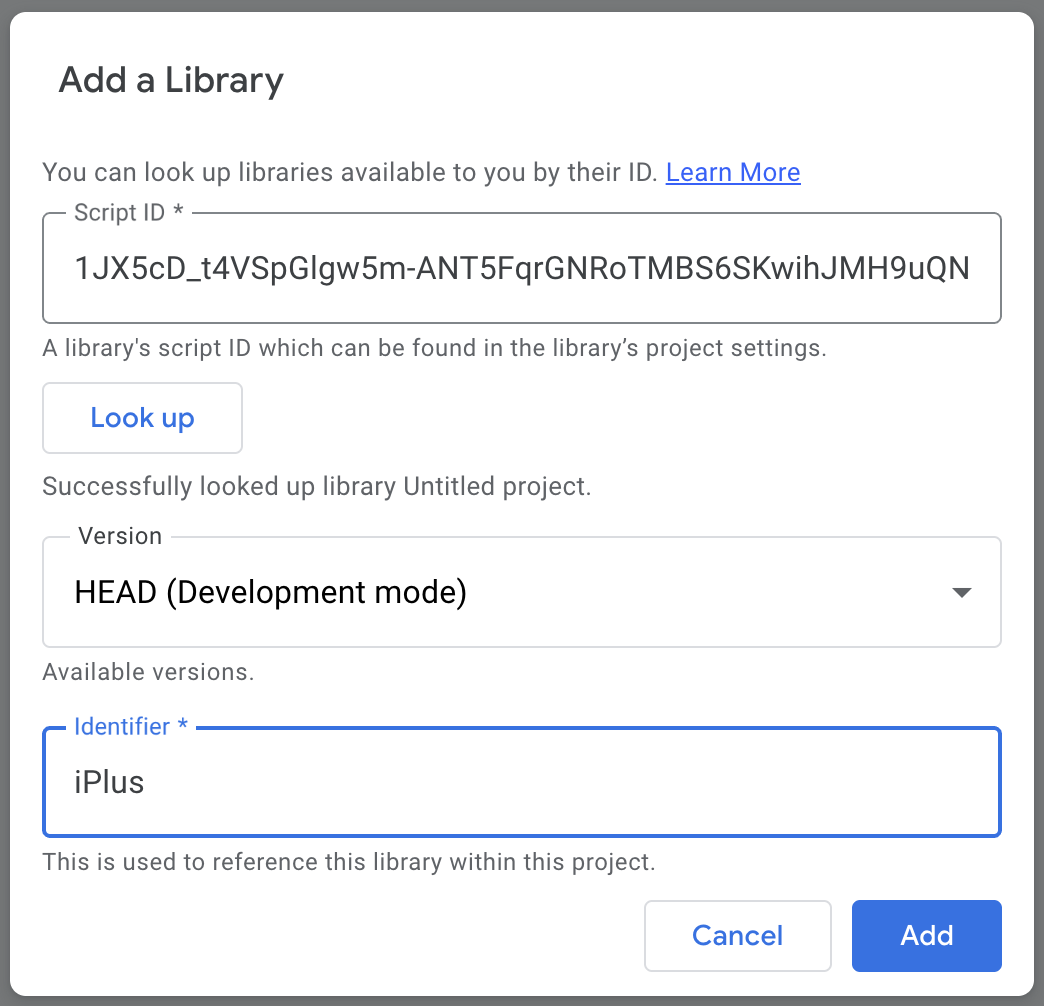
\includegraphics{/images/image3.pdf}

\begin{enumerate}
\def\labelenumi{\arabic{enumi}.}
\setcounter{enumi}{3}
\tightlist
\item
  Leave the version settings as the default HEAD. Change the identifier
  name to ``iPlus'' making sure to maintain the same capitalization.
  Select Add.
\end{enumerate}

\begin{Shaded}
\begin{Highlighting}[]
\NormalTok{iPlus}
\end{Highlighting}
\end{Shaded}

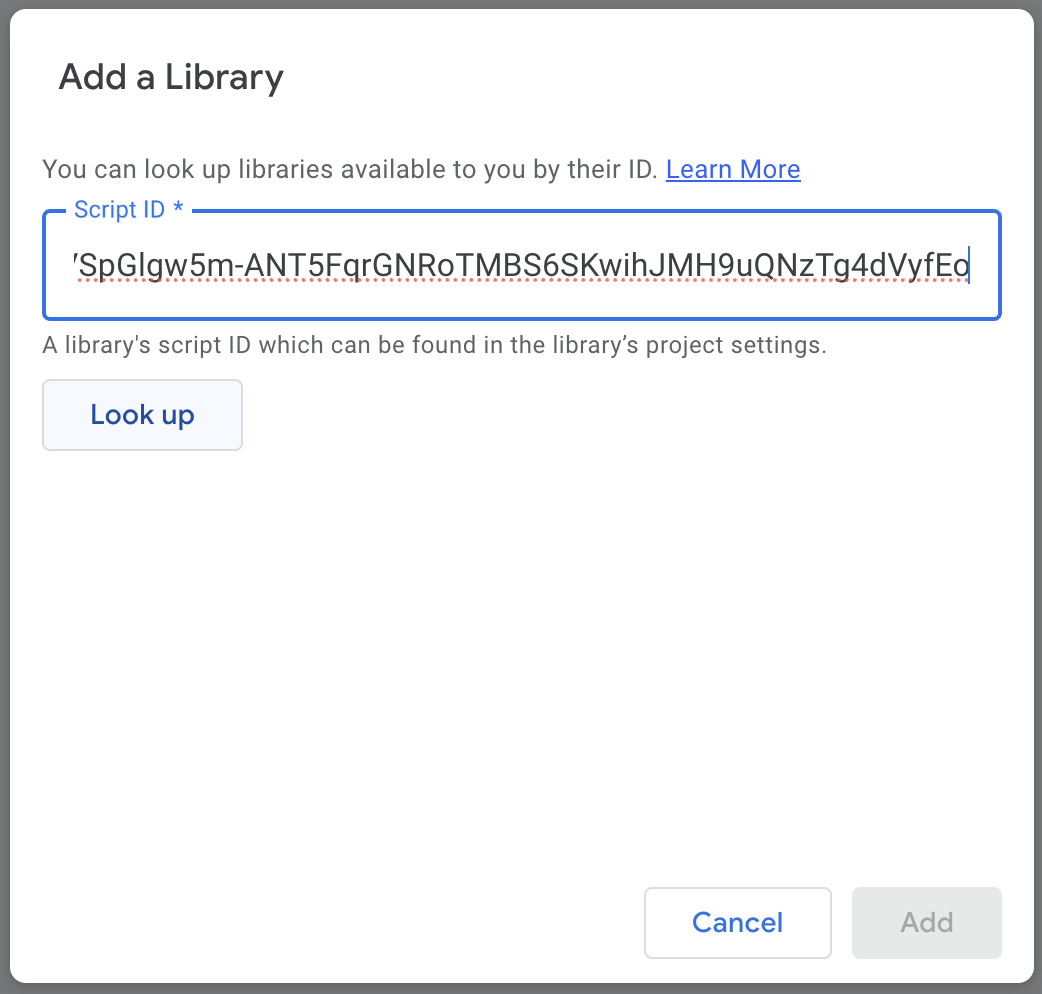
\includegraphics{/images/image4.pdf}

\begin{enumerate}
\def\labelenumi{\arabic{enumi}.}
\setcounter{enumi}{4}
\tightlist
\item
  In the Code.gs file, delete any text that was automatically created
  when creating the Apps Script project. Copy the code below and paste
  it into the Code.gs file. Select the save button to save your changes
  to the project.
\end{enumerate}

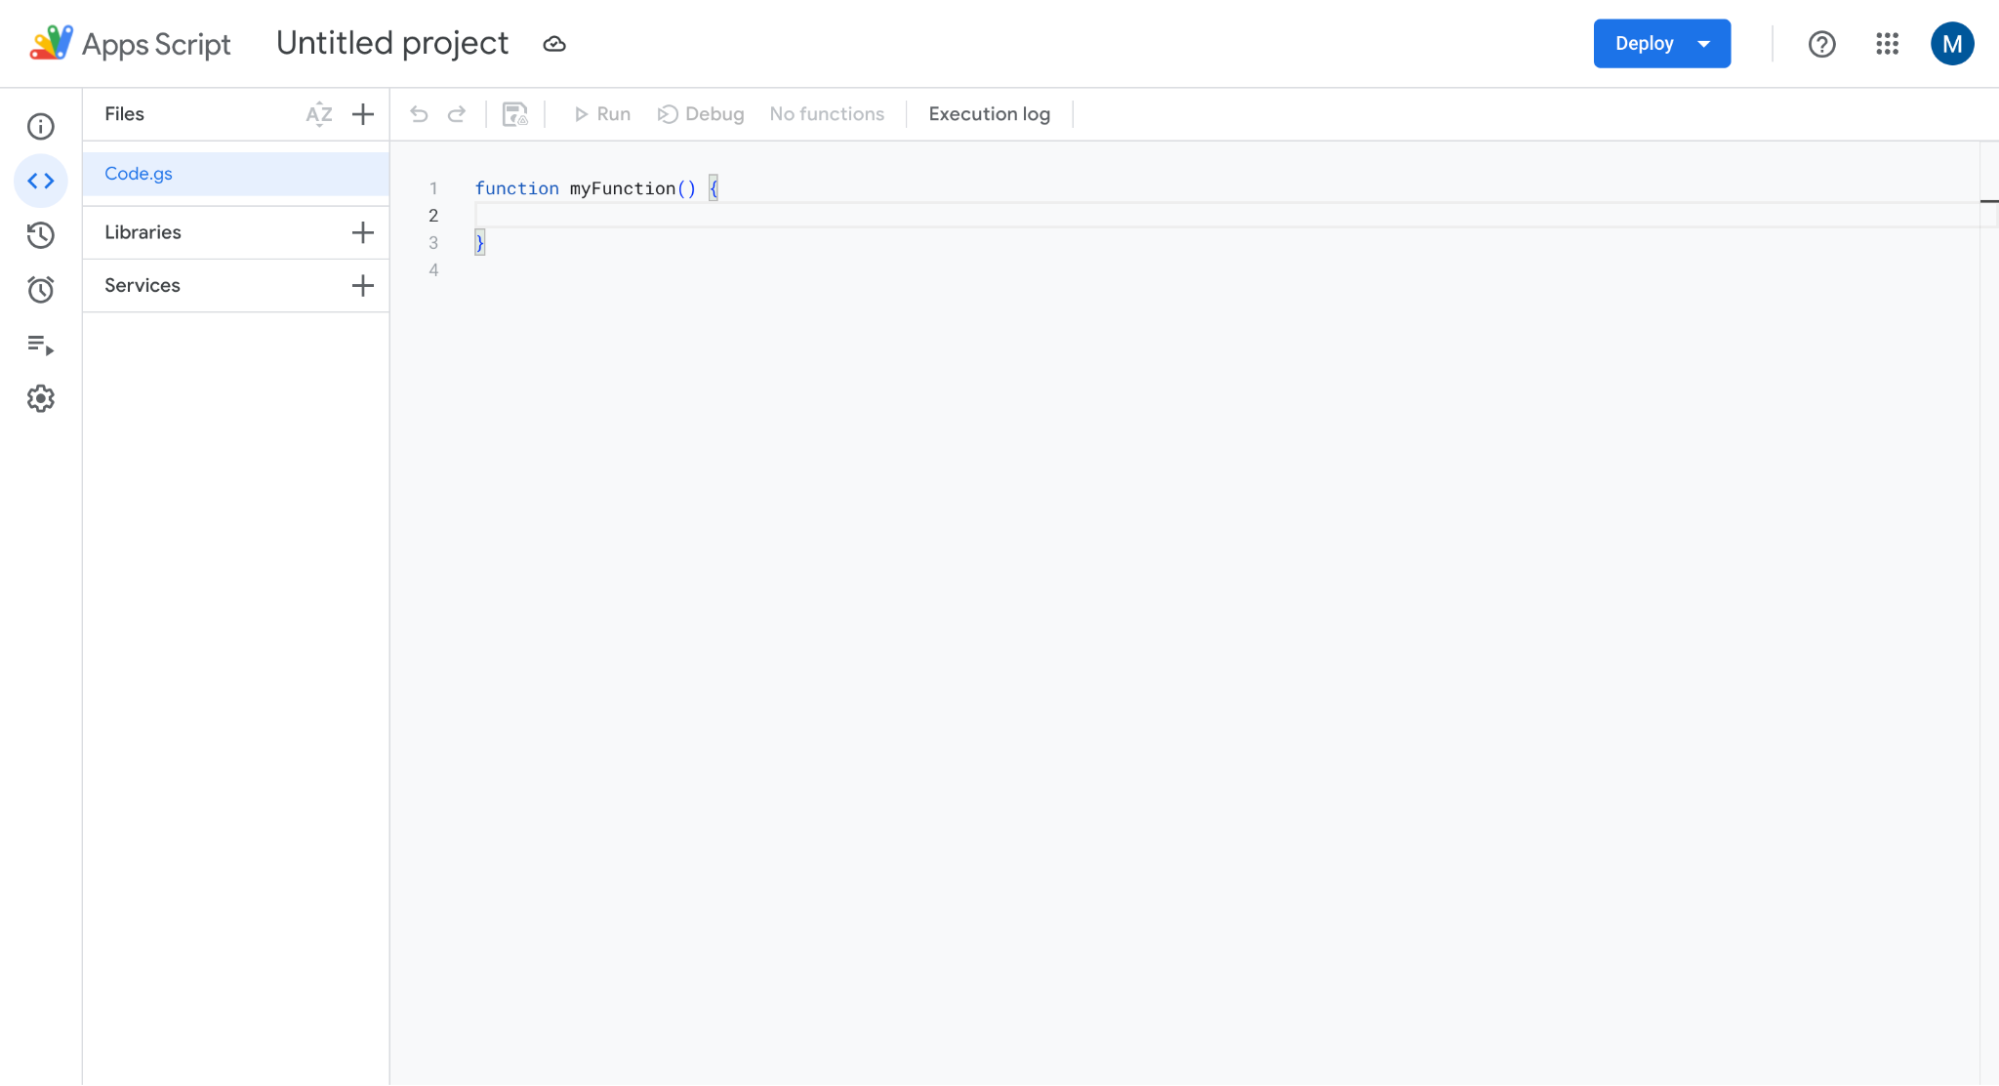
\includegraphics{/images/image6.pdf}

\begin{Shaded}
\begin{Highlighting}[]
\SpecialCharTok{/}\ErrorTok{/}\NormalTok{ DO NOT EDIT THIS EXCEPT TO ADD A CALL TO A FUNCTION}
\ControlFlowTok{function} \FunctionTok{onOpen}\NormalTok{() \{}
\NormalTok{  const ui }\OtherTok{=} \FunctionTok{SpreadsheetApp.getUi}\NormalTok{(); }
  \SpecialCharTok{/}\ErrorTok{/} \SpecialCharTok{{-}{-}{-}{-}{-}{-}{-}{-}{-}{-}{-}{-}{-}{-}{-}{-}{-}{-}{-}{-}{-}{-}{-}{-}{-}{-}{-}{-}{-}{-}{-}{-}{-}{-}{-}{-}}\NormalTok{ CREATE MENU }\SpecialCharTok{{-}{-}{-}{-}{-}{-}{-}{-}{-}{-}{-}{-}{-}{-}{-}{-}{-}{-}{-}{-}{-}{-}{-}{-}{-}{-}{-}{-}{-}{-}{-}{-}{-}{-}{-}{-}}
  \FunctionTok{ui.createMenu}\NormalTok{(}\StringTok{\textquotesingle{}iPlus\textquotesingle{}}\NormalTok{)}
    \FunctionTok{.addItem}\NormalTok{(}\StringTok{\textquotesingle{}Refresh Data\textquotesingle{}}\NormalTok{, }\StringTok{\textquotesingle{}joinSheets\textquotesingle{}}\NormalTok{)}
    \FunctionTok{.addSubMenu}\NormalTok{(}\FunctionTok{ui.createMenu}\NormalTok{(}\StringTok{\textquotesingle{}Pre{-}built Visualizations\textquotesingle{}}\NormalTok{)}
          \FunctionTok{.addItem}\NormalTok{(}\StringTok{\textquotesingle{}Scatterplot: Attendance vs. Score Improvement\textquotesingle{}}\NormalTok{, }\StringTok{\textquotesingle{}preBuiltScatterplot\textquotesingle{}}\NormalTok{)}
          \FunctionTok{.addItem}\NormalTok{(}\StringTok{\textquotesingle{}Boxplot: Race vs. Score Improvement\textquotesingle{}}\NormalTok{, }\StringTok{\textquotesingle{}prebuiltBoxplot\textquotesingle{}}\NormalTok{)}
          \FunctionTok{.addItem}\NormalTok{(}\StringTok{\textquotesingle{}Jitterplot: Score Improvement by Math Teacher\textquotesingle{}}\NormalTok{, }\StringTok{\textquotesingle{}drawTeacherScoreJitterPlot\textquotesingle{}}\NormalTok{))}
    \FunctionTok{.addSubMenu}\NormalTok{(}\FunctionTok{ui.createMenu}\NormalTok{(}\StringTok{\textquotesingle{}Build{-}Your{-}Own Visualizations\textquotesingle{}}\NormalTok{)}
          \FunctionTok{.addItem}\NormalTok{(}\StringTok{\textquotesingle{}Scatterplot\textquotesingle{}}\NormalTok{, }\StringTok{\textquotesingle{}customScatterplot\textquotesingle{}}\NormalTok{)}
          \FunctionTok{.addItem}\NormalTok{(}\StringTok{\textquotesingle{}Boxplot\textquotesingle{}}\NormalTok{, }\StringTok{\textquotesingle{}customBoxplot\textquotesingle{}}\NormalTok{)}
          \FunctionTok{.addItem}\NormalTok{(}\StringTok{\textquotesingle{}Jitterplot\textquotesingle{}}\NormalTok{, }\StringTok{\textquotesingle{}customJitterplot\textquotesingle{}}\NormalTok{))}
    \FunctionTok{.addToUi}\NormalTok{();}

 \SpecialCharTok{/}\ErrorTok{/} \SpecialCharTok{{-}{-}{-}{-}{-}{-}{-}{-}{-}{-}{-}{-}{-}{-}{-}{-}{-}{-}{-}{-}{-}{-}{-}{-}{-}{-}{-}{-}{-}{-}{-}{-}{-}{-}{-}{-}}\NormalTok{ UPDATE IF NEEDED }\SpecialCharTok{{-}{-}{-}{-}{-}{-}{-}{-}{-}{-}{-}{-}{-}{-}{-}{-}{-}{-}{-}{-}{-}{-}{-}{-}{-}{-}{-}{-}{-}{-}{-}{-}{-}{-}{-}{-}}
  \ErrorTok{//}\NormalTok{ check }\ControlFlowTok{if}\NormalTok{ update to merged data is needed}
\NormalTok{  const props }\OtherTok{=} \FunctionTok{PropertiesService.getDocumentProperties}\NormalTok{();}
\NormalTok{  const needsUpdate }\OtherTok{=} \FunctionTok{props.getProperty}\NormalTok{(}\StringTok{"needsUpdate"}\NormalTok{);}
  \FunctionTok{console.log}\NormalTok{()}
  \ControlFlowTok{if}\NormalTok{ (needsUpdate }\SpecialCharTok{==}\ErrorTok{=} \StringTok{"true"}\NormalTok{) \{}
    \SpecialCharTok{/}\ErrorTok{/}\NormalTok{ Example}\SpecialCharTok{:}\NormalTok{ show a toast message}
    \FunctionTok{SpreadsheetApp.getActiveSpreadsheet}\NormalTok{()}\FunctionTok{.toast}\NormalTok{(}\StringTok{"Updates are needed based on recent edits. Please wait until the next message"}\NormalTok{, }\StringTok{"WARNING: Updating \textasciigrave{}Merged Data\textasciigrave{}"}\NormalTok{, }\DecValTok{200}\NormalTok{);}
    \FunctionTok{joinSheets}\NormalTok{();}
    \FunctionTok{SpreadsheetApp.getActiveSpreadsheet}\NormalTok{()}\FunctionTok{.toast}\NormalTok{(}\StringTok{"Updates are finished. You may continue"}\NormalTok{, }\StringTok{"\textasciigrave{}Merged Data\textasciigrave{} update finished"}\NormalTok{, }\DecValTok{200}\NormalTok{);}
\NormalTok{\}}
\NormalTok{\}}


\ControlFlowTok{function} \FunctionTok{onEdit}\NormalTok{(e) \{}
\NormalTok{  const range }\OtherTok{=}\NormalTok{ e.range;}
\NormalTok{  const oldValue }\OtherTok{=}\NormalTok{ e.oldValue;}
\NormalTok{  const newValue }\OtherTok{=} \FunctionTok{range.getValue}\NormalTok{();}

  \ControlFlowTok{if}\NormalTok{ (oldValue }\SpecialCharTok{!=}\ErrorTok{=}\NormalTok{ newValue) \{}
\NormalTok{    const props }\OtherTok{=} \FunctionTok{PropertiesService.getDocumentProperties}\NormalTok{();}
    \FunctionTok{props.setProperty}\NormalTok{(}\StringTok{"needsUpdate"}\NormalTok{, }\StringTok{"true"}\NormalTok{);}
\NormalTok{  \}}
\NormalTok{\}}
\end{Highlighting}
\end{Shaded}

\begin{enumerate}
\def\labelenumi{\arabic{enumi}.}
\setcounter{enumi}{5}
\tightlist
\item
  Select the run button to run i-Plus and integrate it into your Google
  Sheet.
\end{enumerate}

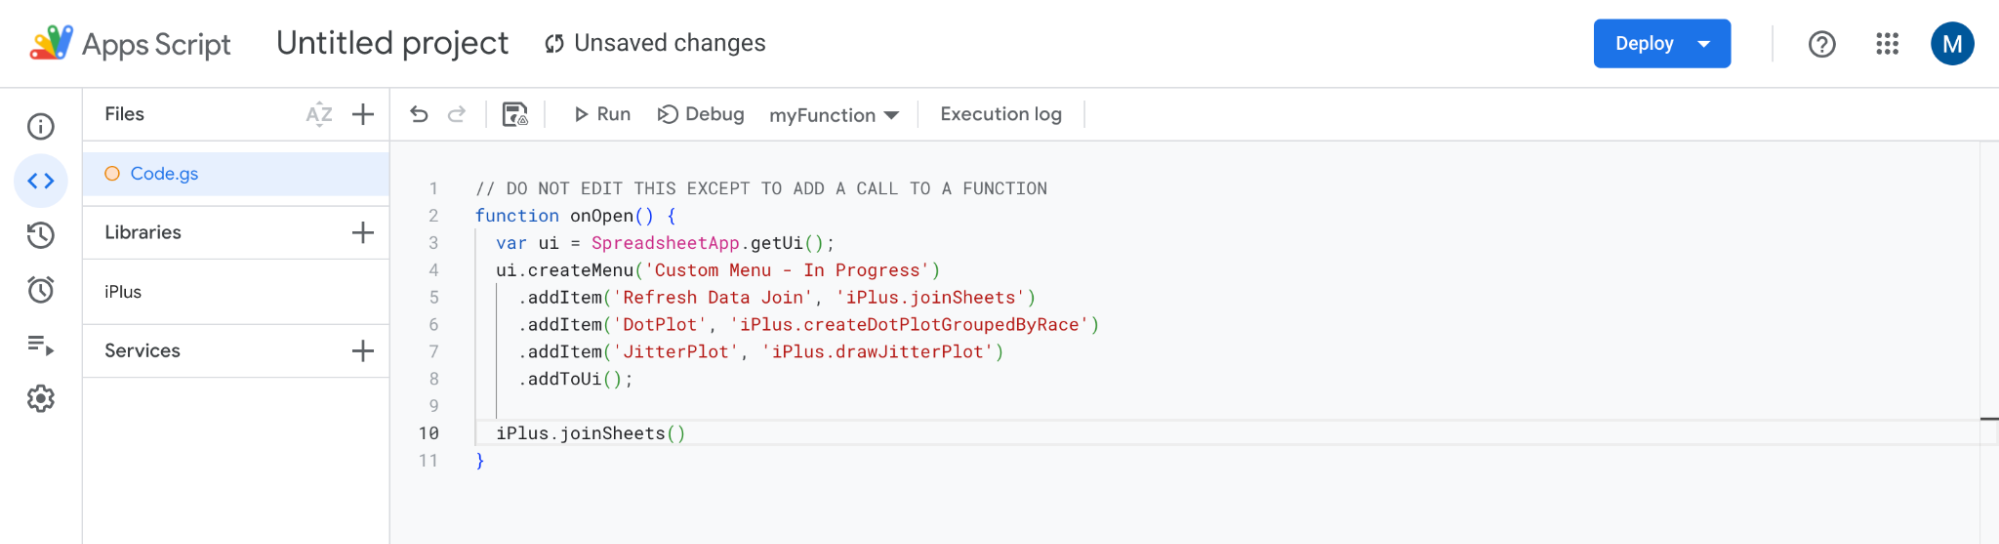
\includegraphics{/images/image5.pdf}

\subsection{Data Management}\label{data-management}

When running i-Plus, certain column headers and sheet names are used to
find the correct data to visualize. Sheet names are most important for
accessing the correct data to visualize. The following sheet names must
stay the same to maintain functionality of i-Plus:

\begin{itemize}
\tightlist
\item
  Elmhurst Data
\item
  6th Grade Math iReady
\item
  7th Grade Math iReady
\item
  8th Grade Math iReady
\end{itemize}

Column headers are most important for creating visualizations contained
in the \textbf{Pre-Built Visualizations} menu within i-Plus. The
following column headers must stay the same to maintain functionality of
these visualizations:

\begin{itemize}
\tightlist
\item
  Race
\item
  Attendance
\item
  Math Teacher
\item
  Initial Scale Score
\item
  Current Scale Score
\end{itemize}

Column order is important for only one column. The column containing
student ID number must be the first column in all of the following
sheets to properly merge i-Ready testing data with Elmhurst demographic
data:

\begin{itemize}
\tightlist
\item
  Elmhurst Data
\item
  6th Grade Math iReady
\item
  7th Grade Math iReady
\item
  8th Grade Math iReady
\end{itemize}

In future iterations of Google Sheets used with i-Plus, please ensure
that these standard sheet names, column headers and column order are
maintained to retain functionality of i-Plus. If the headers are
renamed, custom-built visualizations will still run smoothly, but the
pre-built visualizations will break. If the ID column is not kept as the
first column, both pre-built and custom-built visualizations will break,
and i-Plus will be non-functional.

\subsection{Common Errors}\label{common-errors}

The most common error occurs when trying to join the i-Ready data across
grades. This error may occur when the refresh data functions are
interrupted and not allowed to run in entirety. If this error occurs,
you will receive the following error message as a popup in the sheets
view.

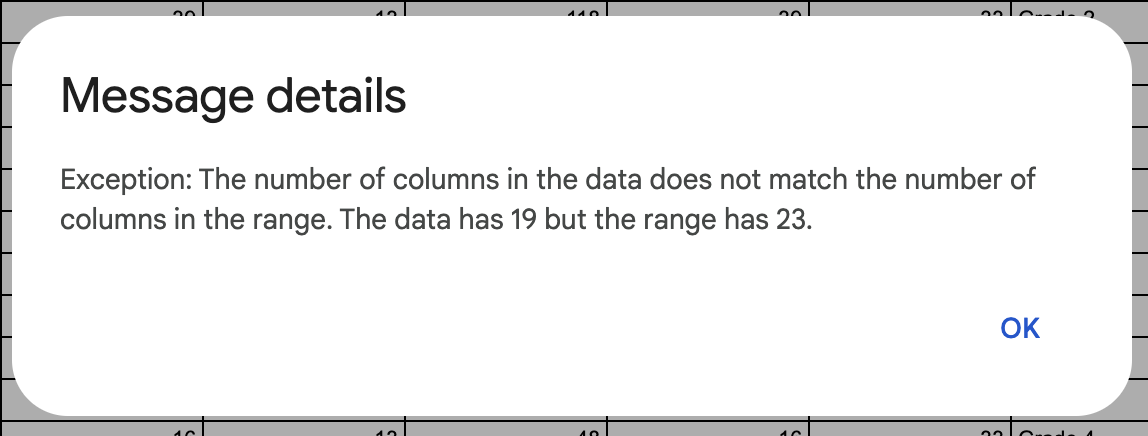
\includegraphics{/images/image8.pdf}

To remedy this error, any transformations to the i-Ready sheets must be
deleted. In the following sheets, delete any column with the header
``Grade'' and ``Score Change'':

\begin{itemize}
\tightlist
\item
  6th Grade Math iReady
\item
  7th Grade Math iReady
\item
  8th Grade Math iReady
\end{itemize}

There may be duplicates of these columns, and any duplicates should also
be deleted, as seen in the following image.

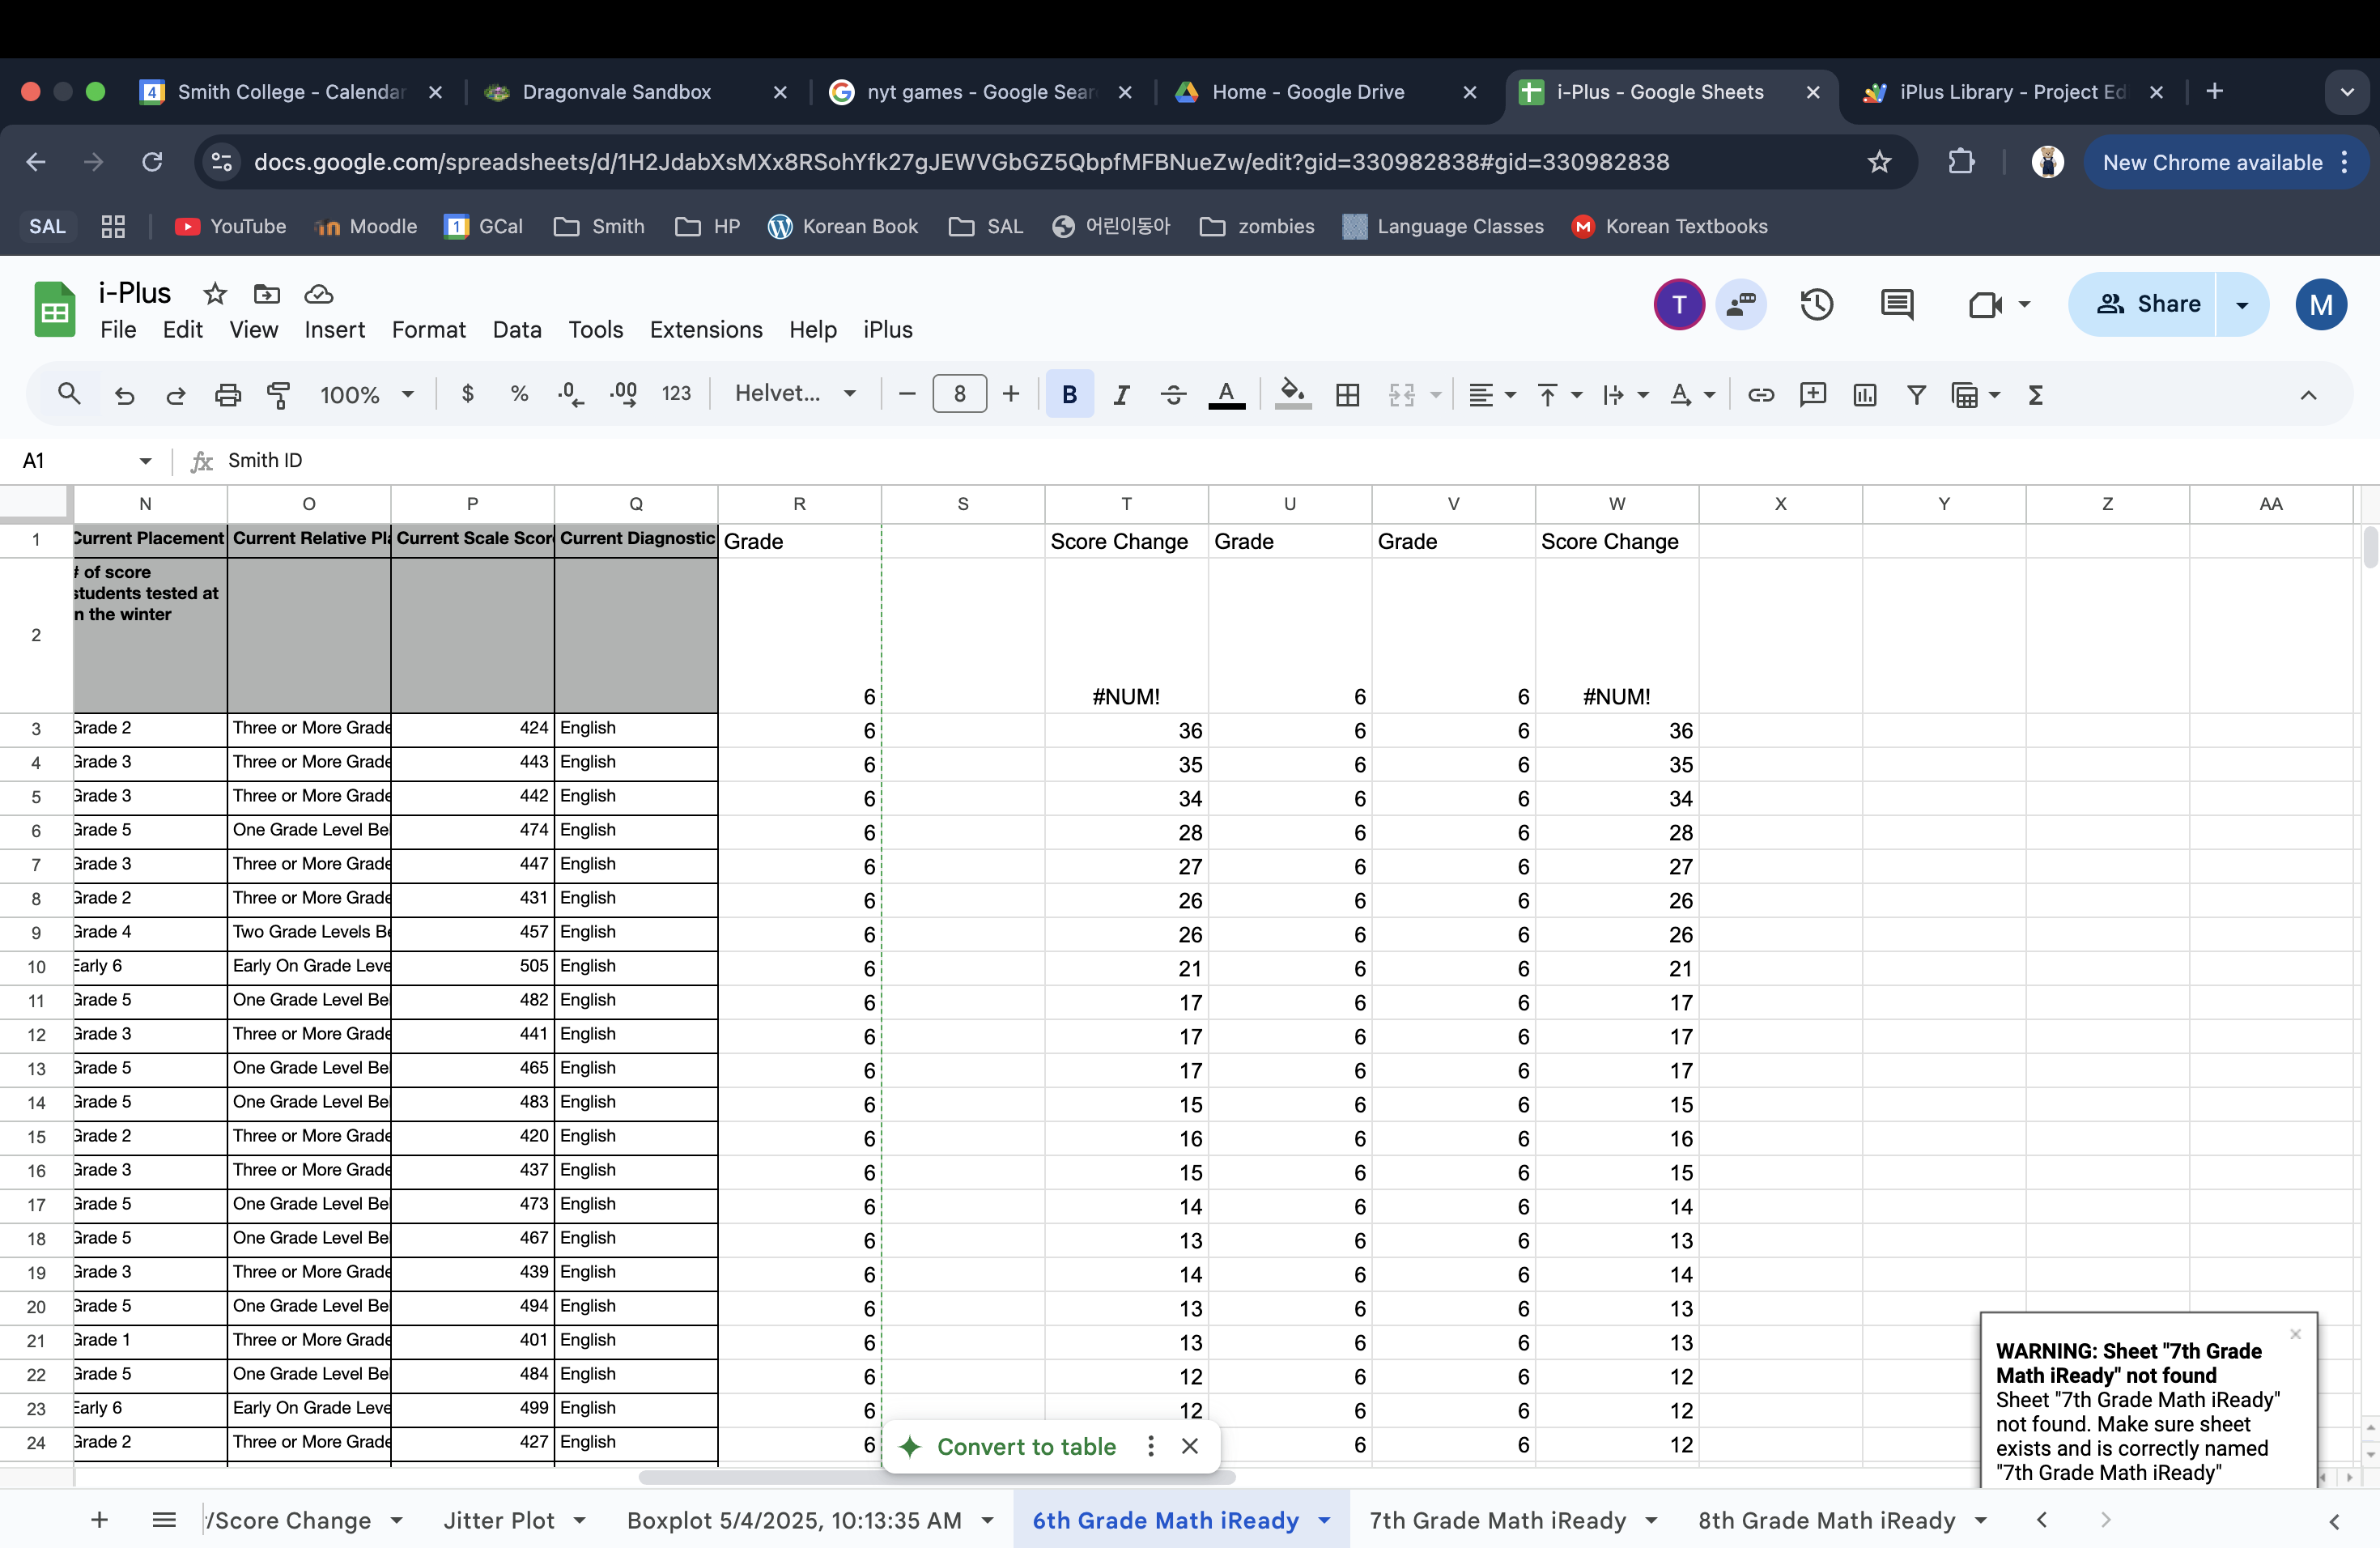
\includegraphics{/images/image9.pdf}




\end{document}
